\documentclass[11pt]{standalone}
\usepackage{pgf, tikz}
\usetikzlibrary{arrows, automata}
\usetikzlibrary{backgrounds}

\begin{document}
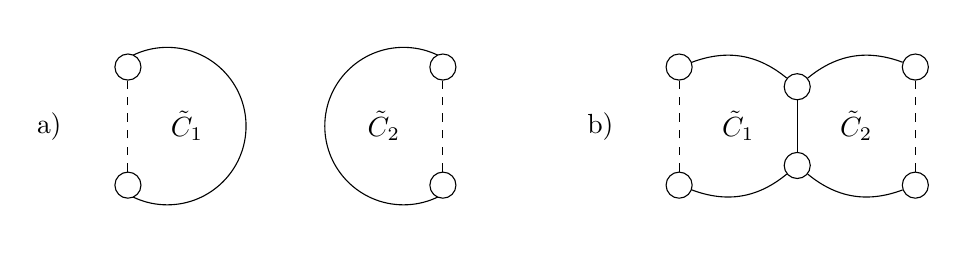
\begin{tikzpicture} [align=center]
\path (-1, 0.75) node (a) {a)}

      (0,0) node[circle, draw, fill = white] (v0) {}
      (0,1.5) node[circle, draw, fill = white] (v1) {}
      (4,0) node[circle, draw, fill = white] (v2) {}
      (4,1.5) node[circle, draw, fill = white] (v3) {}
      
      (0.75, 0.75) node (aC1) {$\tilde{C}_1$}
      (3.25, 0.75) node (aC2) {$\tilde{C}_2$};
      
\draw[dashed] (v0) to (v1);
\draw[dashed] (v2) to (v3);

\begin{scope}[on background layer]
  \clip (0,-0.5) rectangle (4,2);
  \draw (0.5,0.75) circle(1);
  \draw (3.5,0.75) circle(1);
\end{scope}

\path (6, 0.75) node(b) {b)}
      
      (7,0) node[circle, draw] (v4) {}
      (7,1.5) node[circle, draw] (v5) {}
      (8.5,0.25) node[circle, draw] (v6) {}
      (8.5,1.25) node[circle, draw] (v7) {}
      (10,0) node[circle, draw] (v8) {}
      (10,1.5) node[circle, draw] (v9) {}
      
      (7.75,0.75) node (bC1) {$\tilde{C}_1$}
      (9.25,0.75) node (bC2) {$\tilde{C}_2$};
      
\draw[dashed] (v4) to (v5);
\draw (v5) to [bend left] (v7);
\draw (v7) to (v6);
\draw (v6) to [bend left] (v4);
\draw[dashed] (v8) to (v9);
\draw (v8) to [bend left] (v6);
\draw (v7) to [bend left] (v9);

\end{tikzpicture}
\end{document}